% Chapter Template

\chapter{Ensayos y resultados} % Main chapter title

\label{Chapter4} % Change X to a consecutive number; for referencing this chapter elsewhere, use \ref{ChapterX}

%----------------------------------------------------------------------------------------
%	SECTION 1
%----------------------------------------------------------------------------------------

Este capítulo tiene la finalidad de explicar el proceso de aceptación del trabajo y como se determinó que los requerimientos se cumplieron. Además se expone la metodología utilizada para validar el código a medida que se fue escribiendo.

\section{Recursos utilizados}
\label{ch4RecursosUtilizados}

Para desarrollar el trabajo y realizar las pruebas se utilizaron una serie de equipos que se detallan a continuación:

\begin{itemize}
	\item Ordenador portátil Banghó
	\item Ordenador monoplaca Raspberry Pi 4 B
	\item Módulo Nodemcu Esp32 Wi-Fi
	\item Smartphone LG K20 Aurora Black
	\item Router Sagemcom F@ST 3890 v2 TLC
\end{itemize}

Los detalles del ordenador portátil son:

\begin{itemize}
	\item Sistema operativo: Ubuntu 20.04 focal
	\item Kernel: x68\_64 Linux 5.4.0-67-generic
	\item Shell: bash
	\item Resolución: 2732x768
	\item Entorno de escritorio: GNOME 3.36.5
	\item CPU: Intel Core i7-4710MQ @ 8x 3.5GHz
	\item GPU: Intel Corporation 4th Gen Core Processor Integrated Graphics Controller (rev 06)
	\item RAM: 11891MiB
\end{itemize}

Se utilizaron además una serie de programas para hacer el desarrollo y las pruebas y se los enumera a continuación:

\begin{itemize}
	\item Visual Studio Code versión 1.54.3
	\item Navegador Chromium versión 89.0.4389.90 (Build oficial) snap (64 bits)
	\item Terminal de Gnome versión 3.36.2
	\item Postman versión 8.0.7
	\item Wireshark versión 3.2.3
	\item Nmap versión 7.80
	\item Mosquitto versión 1.6.9
\end{itemize}

% Explicación del proceso de decición para determinar cuando debí realizar scripts. Descripción de las scripts creados y su valides
\section{Guiones y comandos}
% necesidad de realizar mocks
En el capítulo \ref{Chapter3} se detalló el trabajo realizado, como funcionan todas sus partes y la interdependencia que existe entre ellas.
Pero antes de llegar a tener un sistema completo y funcionando se tuvieron partes incompletas y servicios inexistentes.
Esta situación demandó crear una serie de guiones y comandos que pudieran recrear de forma limitada alguna de las funcionalidades de las dependencias de cada componente.

\subsection{Base de datos}

Varios de los servicios necesitaron tener acceso a una conexión de base de datos en MongoDB durante su desarrollo.
Para crear una instancia efímera del motor se utilizó un guión de bash que se puede ver en el código \ref{cod:ch3GuionDB}.
En él se puede observar que se utilizó docker para esa etapa del trabajo.
El código se escribió para facilitar las modificaciones en su configuración y se designó una carpeta para almacenar una serie de archivos en JavaScript.
Estos archivos cumplieron la función de poblar con datos a MongoDB.

\begin{lstlisting}[language=bash,label=cod:ch3GuionDB,caption=Guión de base de datos.]
#!/bin/bash
IMAGE_NAME=mongo
CONTAINER_NAME=mongo
CONTAINER_PORT=27017
CONTAINER_DIRECTORY=/scripts
MACHINE_PORT=27017
MACHINE_DIRECTORY=$PWD/mockDB

docker run \
--rm \
--name $CONTAINER_NAME \
-p $MACHINE_PORT:$CONTAINER_PORT \
-v $MACHINE_DIRECTORY:$CONTAINER_DIRECTORY \
-d \
$IMAGE_NAME

sleep 5
docker exec $CONTAINER_NAME sh -c "mongo < /scripts/mockData.js"
\end{lstlisting}

\subsection{Mosquitto}

Los servicios que necesitaron de un \emph{broker} MQTT para validar su desarrollo se valieron de un guión de bash.
Ese guión, que se puede ver en el código \ref{cod:ch3GuionMosquitto}, se encargó de proveer un \emph{broker} completamente promiscuo y sin ninguna medida de seguridad.
La razón para generar esta configuración fue eliminar cualquier tipo de falla producto de las medidas de seguridad.
De esta manera cualquier comportamiento no deseado se origina en el código escrito para cada servicio en particular.

\begin{lstlisting}[language=bash,label=cod:ch3GuionMosquitto,caption=Guión de Mosquitto.]
#!/bin/bash
IMAGE_NAME=eclipse-mosquitto
CONTAINER_NAME=mosquitto
CONTAINER_PORT=1883
MACHINE_PORT=1883

docker run \
--rm \
--name $CONTAINER_NAME \
-p $MACHINE_PORT:$CONTAINER_PORT \
-d \
$IMAGE_NAME
\end{lstlisting}

Se utilizaron los servicios que provee Mosquitto para realizar publicaciones y subscripciones.
Estas acciones fueron hechas desde la terminal del ordenador portátil y del ordenador monoplaca.
Los comandos se pueden ver de forma genérica en el código \ref{cod:ch3ComandosMosquitto}.

\begin{lstlisting}[language=bash,label=cod:ch3ComandosMosquitto,caption=Comandos de Mosquitto.]
mosquitto_sub -h 'localhost' -u 'docker' -P 'container' -t 'data/#'
mosquitto_pub -h 'localhost' -u 'device' -P 'thing' -t 'data' -m 'edu-ciaa,25'
\end{lstlisting}

\subsection{Redis}

Los componentes del sistema que utilizaron un mecanismo de identificación de clientes usaron Redis para lograrlo.
Por ese motivo se creó un guión de bash que creara un contenedor de Redis con su configuración por defecto.
El código \ref{cod:ch3GuionRedis} muestra las instrucciones necesarias para lograr el objetivo.
Se puede ver en su última línea que se creó un token de prueba para verificar la conexión con el servicio.

\begin{lstlisting}[language=bash,label=cod:ch3GuionRedis,caption=Guión de Redis.]
#!/bin/bash
IMAGE_NAME=redis
CONTAINER_NAME=redis
CONTAINER_PORT=6379
MACHINE_PORT=6379

docker run \
--rm \
--name $CONTAINER_NAME \
-p $MACHINE_PORT:$CONTAINER_PORT \
-d \
$IMAGE_NAME

sleep 5
docker exec redis sh -c "redis-cli SET xxxx.yyyy.zzzz 3"
\end{lstlisting}

\newpage

\subsection{Nodejs}
Se necesitó crear un ambiente de desarrollo y pruebas para podes escribir el código de los servicios basados en Nodejs.
Esto se logró al construir los componentes que se detallan a continuación:

%\newpage

\begin{itemize}
	\item Archivo de variables de entorno
	\item Archivo de configuración del framework de pruebas Mocha
	\item Creación de guiones en el archivo de paquetes de Nodejs
\end{itemize}

El archivo de variables de entorno se utilizó para no colocar en el código las contraseñas ni las direcciones de los recursos externos.
Un ejemplo de este tipo de archivo se puede ver en el código \ref{cod:ch3VariablesEntorno}.
Su configuración apunta a servicios creados con los comandos y guiones de pruebas.
La ventaja de esta metodología es que se puede usar el mismo código en producción y durante las pruebas.

\begin{lstlisting}[language=bash,label=cod:ch3VariablesEntorno,caption=Archivo de variables de entorno.]
PORT=8080
DB_URL=mongodb://localhost:27017/gador
REDIS_HOST=127.0.0.1
REDIS_PORT=6379
SECRET_KEY=secret
TIME_TO_LIVE=120
MQTT_HOST=mqtt://localhost
\end{lstlisting}

Para configurar el framework de pruebas de Mocha se utilizó la configuración del código \ref{cod:ch3ConfiguraciónMocha}.
Se observa que se determinó un tiempo de ejecución máximo para evitar bloquear el ensayo.
La contingencia se puede dar en el caso que una función no pueda converger a un resultado.

\begin{lstlisting}[language=bash,label=cod:ch3ConfiguraciónMocha,caption=Configuración de Mocha.]
module.exports = {
    recursive: true,
    slow: 75,
    timeout: 5000,
    spec: ['test/**/*.test.js']
}
\end{lstlisting}

Finalmente se crearon guiones para correr con el gestor de paquetes de Nodejs.
Se los puede ver en el código \ref{cod:ch3GuionesNodejs} y los guiones a analizar son los siguientes:

\begin{itemize}
	\item dev
	\item test
\end{itemize}

El guión dev cumple la función de correr los guiones de creación de MongoDB, Redis y Mosquitto.
Además carga las variables de entorno en la sesión de terminal para finalmente correr la aplicación en modo desarrollo.
Con el entorno de desarrollo activo se pueden realizar las pruebas al ejecutar el guión test.
Este guión limpia la terminal y reinicia la base de datos. Luego procede a cargar las variables de entorno y ejecutar Mocha.

\begin{lstlisting}[language=bash,label=cod:ch3GuionesNodejs,caption=Guiones de Nodejs.]
"build": "npm install",
"dev": "./mockDB/mongo.sh && ./mockDB/redis.sh && ./mockDB/mosquitto.sh && eval $(cat ./.env) nodemon ./src/app.js",
"production": "eval $(cat ./enviroment/.env) node ./src/app.js",
"test": "clear && ./mockDB/restart.sh && eval $(cat ./.env) mocha",
"clean": "docker stop mongo && docker stop redis && docker stop mosquitto"
\end{lstlisting}

% Explicación de como se implementó TDD en algunos servicios y como se hicieron pruebas unitarias en otras
\section{Pruebas unitarias}
% introducción. Inicio con TDD, abandono de TDD por incremento exponencial en la complejidad de las pruebas.
Durante las primeras etapas del desarrollo del trabajo se utilizó la metodología \emph{Test Driven Development (TDD)}.
Luego se la abandonó y se pasó a utilizar distintos programas para realizar las pruebas.
Se decidió realizar el cambio en la forma de trabajar debido a que la complejidad de las pruebas fue creciendo de manera exponencial.
Se llegó a un punto del trabajo donde \emph{TDD} se volvió improductivo y su abandono fue la única manera de continuar a un ritmo de avance aceptable.

En la primera etapa del trabajo se escribieron pruebas unitarias que fueron creciendo a medida que se agregaban funcionalidades al código fuente.
En el caso del \emph{endpoint} que representa los dispositivos en el Backend el archivo de pruebas unitarias alcanzó las 285 líneas de código.
Mientras que el archivo del \emph{endpoint} solo demandó 148 líneas.
Se alcanzó el punto donde la extensión de las pruebas superaron al código fuente.
Algunos ejemplos de pruebas de la entidad dispositivos del Backend se puede ver en el código \ref{cod:ch3BackendUnitTest}.
El ejemplo se divide en cuatro pruebas realizadas al método \emph{GET} de la entidad cuando se solicita un dispositivo en particular.
Los casos analizados son:

\begin{itemize}
	\item El pedido no tiene credenciales
	\item El pedido tiene credenciales inválidas
	\item El pedido tiene credenciales válidas y el dispositivo existe
	\item El pedido tiene credenciales válidas y el dispositivo no existe
\end{itemize}

\begin{lstlisting}[language=bash,label=cod:ch3BackendUnitTest,caption=Extracto de prueba unitaria Backend.]
describe(`GET on "${url}/<device tag>" without a token`, () => {
    it('should return STATUS 401', async () => {
        let response = await fetch(`${url}/esp32`, voidGET);
        expect(response.status).to.be.equal(401);
    });
});

describe(`GET on "${url}/<device tag>" with an INVALID token`, () => {
    it('should return STATUS 401', async () => {
        let response = await fetch(`${url}/esp32`, invalidGET);
        expect(response.status).to.be.equal(401);
    });
});

describe(`GET on "${url}/<device tag>" with a VALID token`, () => {
    let data = { serial: 123, tag: "esp32", modbus: 0, frec: 60, unit: "t" };
    data = JSON.stringify(data);
    it('should return "status 200" and data', async () => {
        let response = await fetch(`${url}/esp32`, validGET);
        let status = response.status;
        let text = await response.text();
        expect(status).to.be.equal(200);
        expect(text).to.be.equal(data);
    });
});

describe(`GET on "${url}/<device tag>" when the device does not exist`, () => {
    it('should return "status 204"', async () => {
        let response = await fetch(`${url}/void`, validGET);
        let status = response.status;
        expect(status).to.be.equal(204);
    });
});
\end{lstlisting}

Este procedimiento de pruebas se generó para cada función de cada entidad.
Razón por la cual los archivos de pruebas unitarias crecieron rápidamente.
Cuando se abandonó \emph{TDD} se usaron programas como \emph{Postman} para hacer pruebas manuales de casos puntuales.
En la imagen \ref{fig:ch4Postman1} se visualiza la operación realizada para obtener las credenciales necesarias.
La ilustración \ref{fig:ch4Postman2} muestra la creación exitosa de una sesión.
En la figura \ref{fig:ch4Postman3} se observa el uso de las credenciales para hacer un pedido de dispositivos al Backend.
Finalmente en la imagen \ref{fig:ch4Postman4} se ve la respuesta obtenida. 


\begin{figure}[h]
	\centering
	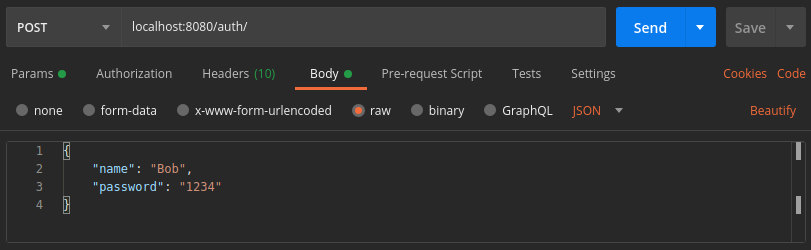
\includegraphics[width=\textwidth]{./Figures/postman1.png}
	\caption{Pedido de credenciales con Postman.}
	\label{fig:ch4Postman1}
\end{figure}

\begin{figure}[h]
	\centering
	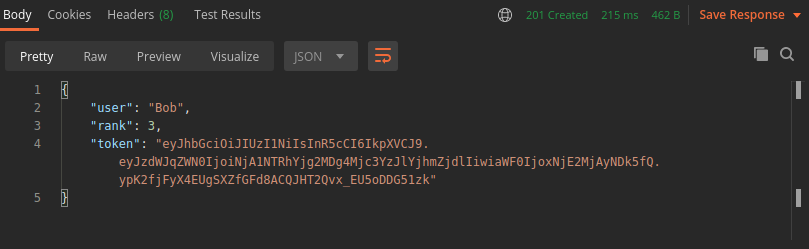
\includegraphics[width=\textwidth]{./Figures/postman2.png}
	\caption{Respuesta de credenciales con Postman.}
	\label{fig:ch4Postman2}
\end{figure}

\begin{figure}[h]
	\centering
	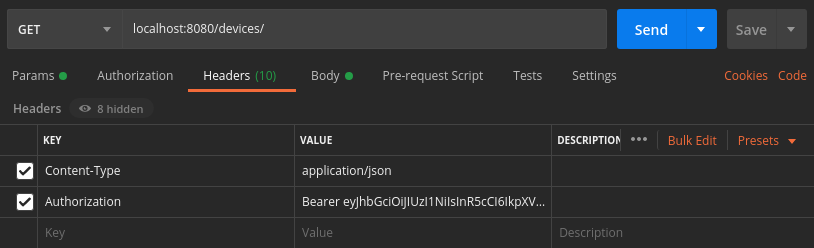
\includegraphics[width=\textwidth]{./Figures/postman3.png}
	\caption{Pedido de dispositivos con Postman.}
	\label{fig:ch4Postman3}
\end{figure}

\begin{figure}[h]
	\centering
	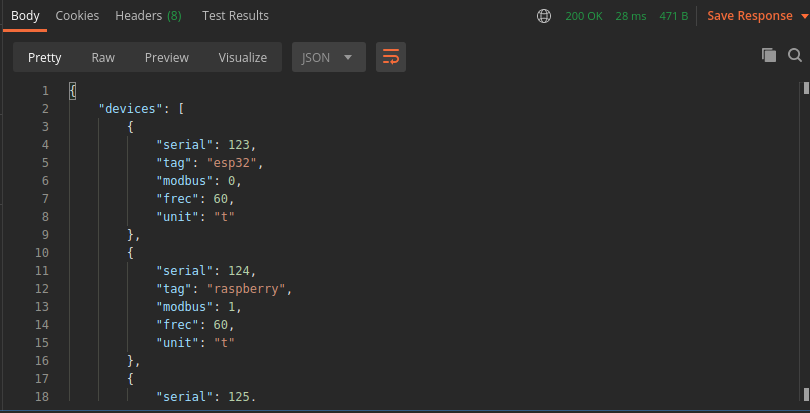
\includegraphics[width=\textwidth]{./Figures/postman4.png}
	\caption{Respuesta de dispositivos con Postman.}
	\label{fig:ch4Postman4}
\end{figure}

% Explicación del proceso de decición para determinar cuando debí realizar simulaciones. Descripción de las simulaciones creadas y su valides
\section{Simulaciones}
El trabajo debe interactuar con entidades externas como se indicó en la sección \ref{ch3Arq} y se puede ver en la figura \ref{fig:ch3EsquemaTrabajo}.
Para validar el comportamiento con estos agentes se necesitó crear simulaciones que tomaran el rol de dispositivos, usuarios y del servidor EBI.

Las funcionalidades de EBI se simularon con el código \ref{cod:ch4SimulacionEBI} escrito en Python.
Cuando se invoca el programa se realizan lecturas y escrituras de los registros del servidor Modbus dentro de Nodos.

\begin{lstlisting}[language=python,label=cod:ch4SimulacionEBI,caption=Simulación de EBI.]
from pyModbusTCP.client import ModbusClient
import random

def r():
    return random.randint(0, 65535)

client = ModbusClient(host='0.0.0.0', port=5020,
                      auto_open=True, auto_close=True)

regs = client.read_holding_registers(0, 10)

if regs:
    print('Holding Registers: ' + str(regs))
else:
    print('reading error')

if client.write_multiple_registers(0, [r(), r(), r(), r(), r(), r(), r(), r(), r(), r()]):
    print('writing successful')
else:
    print('writing error')
\end{lstlisting}

El usuario fue simulado utilizando un smartphone y se le solicitó a terceros que interactuaran con el sistema.
Con el objetivo de probar la experiencia de uso y la facilidad para manejar el flujo de la aplicación.

Finalmente el dispositivo fue simulado con un modulo Nodemcu Esp32 Wi-Fi que entrega valores aleatorios en intervalos regulares.
En el código \ref{cod:ch4SimulacionDispositivo} se detalla la función de envío de datos.
Se tiene la posibilidad de usar los \emph{topics} DATA y LIVE, para persistir en la base de datos o realizar calibraciones respectivamente.

\begin{lstlisting}[label=cod:ch4SimulacionDispositivo,caption=Función de envío de datos.]
void send_data()
{
  String temperature = String(random(MIN_TEMPERATURE, MAX_TEMPERATURE));
  String my_message = String(DEVICE + temperature);
  if (direction == 0)
  {
    mqtt.publish(DATA, my_message.c_str());
  }
  else
  {
    mqtt.publish(LIVE, my_message.c_str());
  }

  delay(frec);
}
\end{lstlisting}

% Recepción del cliente, sus comentarios y modificaciones realizadas para satisfacerlo
\section{Pruebas del cliente}

El cliente realizó las pruebas que validan la comunicación del sistema con EBI.
Para ese fin utilizó una máquina virtual con una licencia de prueba de seis horas que otorgó generosamente la empresa Honeywell.
No fue posible probarlo en el ambiente productivo real debido a las políticas de seguridad de Gador.

Finalmente se realizó una demostración final a un representante del departamento de ingeniería de Gador.
En ese evento se mostró todo el código y las funcionalidades.
Se logró nn esa instancia que el cliente diera su aprobación y conformidad.
Con este último paso se finalizó el desarrollo del trabajo y se aceptó que se cumplieron con todos los requerimientos.
